\section{Theorie}
\label{sec:Theorie}
\subsection{Allgemeines zur Wärmepumpe}
Zu Betrachten sind zwei Wärmereservoire mit verschiedener Temperatur.
Zwischen diesen findet Wärmeübertragung ohne äußere Einwirkung stets vom
wärmeren zum kälteren Wärmereservoir statt. Dies ist eine mögliche Formulierung des
zweiten Hauptsatzes der Thermodynamik oder kann alternativ in anderen Formulierungen
durch diese gezeigt werden. \newline
Eine Wärmepumpe ermöglicht durch Aufwendung mechanischer Energie den Transport von
thermischer Energie vom kälteren zum wärmeren Reservoir.
Eine Skizze zur Veranschaulichung der Funktionsweise einer Wärmepumpe ist in
Abbildung \ref{fig:waermepumpebild} zu sehen. Die Bezeichnungen in der Skizze werden
wie folgt umbenannt:
\begin{align*}
p_\text{warm} &\coloneqq p_\text{b} & p_\text{kalt} &\coloneqq p_\text{a} \\
T_\text{warm} &\coloneqq T_1 & T_\text{kalt} &\coloneqq T_2
\end{align*}

\begin{figure}[H]
  \centering
  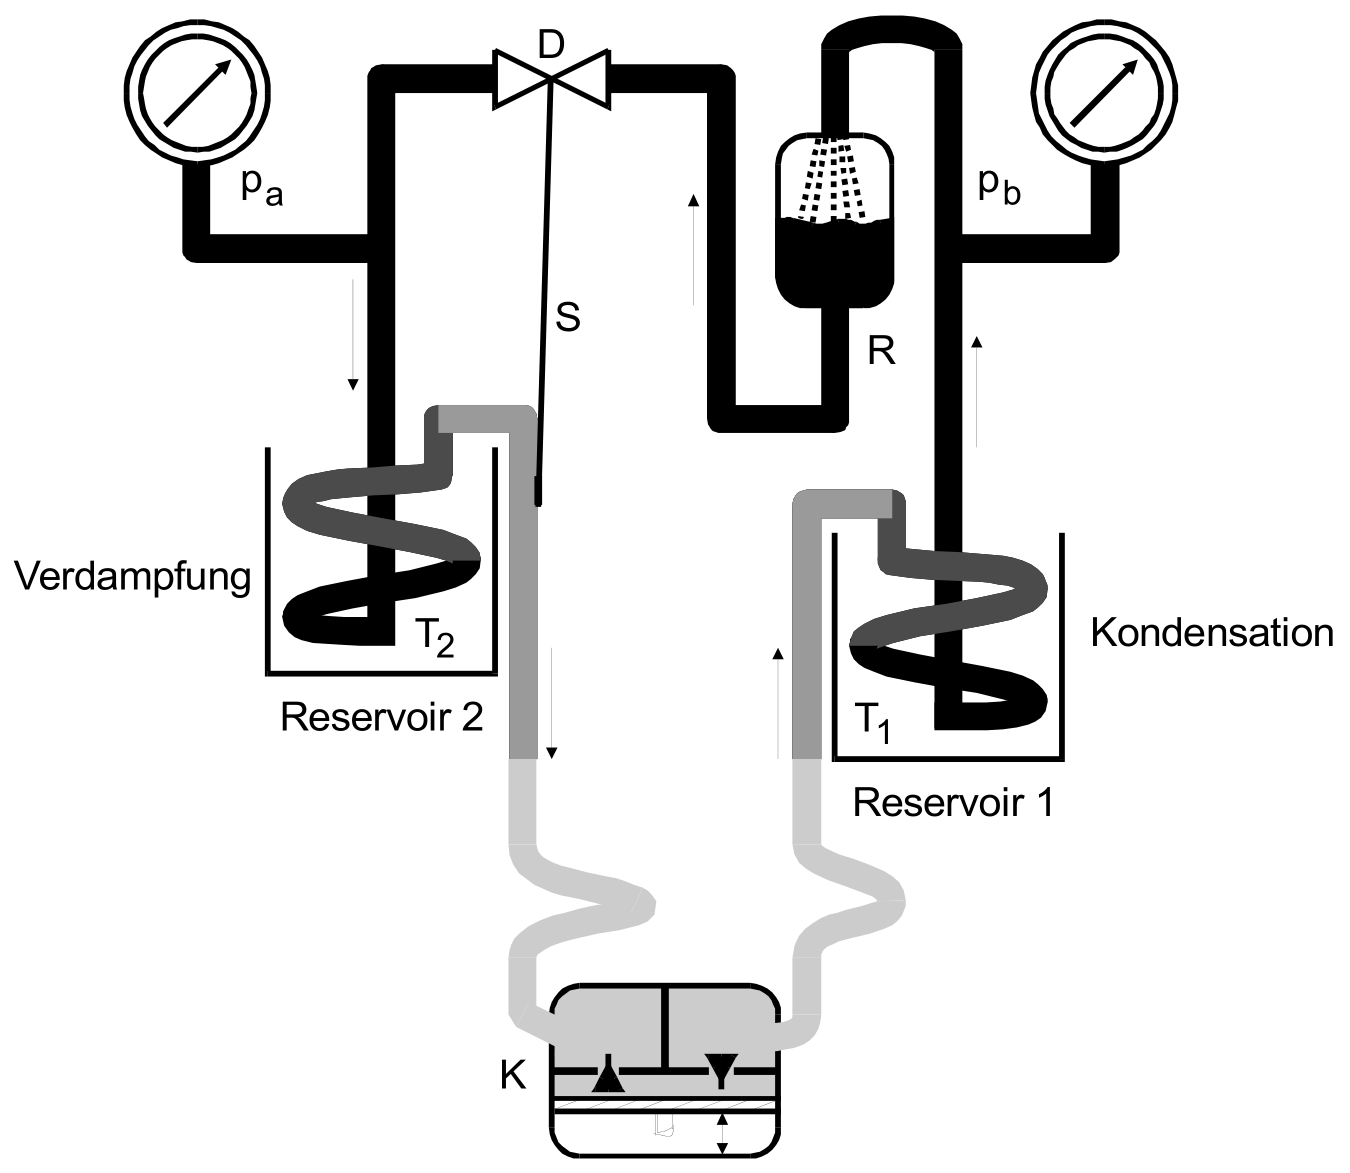
\includegraphics[width=250pt]{data/waermepumpe.png}
  \caption{Skizze einer Wärmepumpe, es gilt $p_\text{warm} > p_\text{kalt}$ und $T_\text{warm} > T_\text{kalt}$ \cite{Versuchsanleitung}}
  \label{fig:waermepumpebild}
\end{figure}

Ein reales Gas durchläuft die Wärmepumpe als Transportmedium. Dieses nimmt beim Verdampfen
Wärme auf und gibt sie bei Verflüssigung wieder ab, sodass die transportierte Wärme
als Phasenumwandlungsenergie des verwendeten Gases vorliegt. Der Kompressor K ermöglicht
einen Kreislauf des Gases durch die Wärmepumpe. Das Gas ist bei der Temperatur $T_\text{warm}$
und dem Druck $p_\text{warm}$ flüssig und liegt bei der Temperatur $T_\text{kalt}$ und dem
Druck $p_\text{kalt}$ im gasförmigen Aggregatzustand vor. Reservoir 2 ist hier das
kältere Reservoir, welches Reservoir 1 wärmt. Das flüssige Gas durchströmt die Stelle D
und verdampft im Reservoir 2. Dabei wird dem dort befindlichen Stoff die Verdampfungswärme
$L_m$ pro Gramm entzogen. Daraufhin wird das Medium im Kompressor adiabatisch komprimiert,
sodass Temperatur und Druck steigen. In Reservoir 1 verflüssigt sich das Gas, indem es
die gleiche Wärmemenge, die es in Reservoir 2 aufgenommen hat, wieder abgibt.
Die restlichen Bestandteile der Apparatur und die Steuereinrichtungen D, S und R sind
ansonsten nicht weiter für die prinzipielle Funktionsweise der Wärmepumpe relevant.

\subsection{Die Güteziffer einer Wärmepumpe}
Wird der erste Hauptsatz der Thermodynamik auf das System einer Wärmepumpe angewandt,
so erhält man die Beziehung
\begin{equation}
  Q_\text{warm} = Q_\text{kalt} + A\,.
  \label{eqn:waermebilanz}
\end{equation}
Dabei ist $Q_\text{warm}$ die dem wärmeren Reservoir zugeführte Wärme,
$Q_\text{kalt}$ die dem kälteren Reservoir entnomenne Wärme und $A$ die aufgewandte
mechanische Arbeit.
Die Größe
\begin{equation}
  \nu = \frac{Q_\text{warm}}{A}
  \label{eqn:defnu}
\end{equation}
wird als Güteziffer der Wärmepumpe bezeichnet.
Erfolgt die Wärmeübertragung idealisiert vollständig reversibel, so gilt für die ideale
Güteziffer auch
\begin{equation}
  \nu_\text{id} = \frac{T_\text{warm}}{T_\text{warm} - T_\text{kalt}}\,.
  \label{eqn:nuid}
\end{equation}
Bei einer realen Wärmepumpe liegt ein irreversibler thermodynamischer Prozess vor,
sodass die reale Güteziffer $\nu_\text{real}$ stets echt kleiner als die ideale
Güteziffer ist.
Gleichung \eqref{eqn:nuid} zeigt, dass eine Wärmepumpe effizient arbeitet und damit
die Güteziffer groß wird, wenn die Temperaturdifferenz der Reservoire
klein wird. Dies stellt einen Vorteil gegenüber Verfahren dar, bei denen mechanische Arbeit
direkt in Wärme umgewandelt wird, denn dabei ist die erhaltene Wärmemenge stets kleiner
oder gleich der aufgewandten mechanischen Arbeit.\\
Um die reale Güteziffer zu ermitteln, wird die Wärmekapazität der Substanz
in Reservoir 1 benötigt. Diese wird mit $m_1 c_\text{W}$ bezeichnet, da in der konkreten Durchführung
Wasser verwendet wird. Außerdem ist die Kenntnis der Wärmekapazität $m_\text{k} c_\text{k}$
der Apparatur, hier konkret bestehend aus einem Eimer und der Kupferschlange, erforderlich.
Für die als Differenzenquotient ausgedrückte gewonnene Wärmemenge pro Zeitintervall
folgt aus einer Messreihe der Temperatur $T_\text{warm}$ in Abhängigkeit der Zeit $t$
\begin{equation}
  \frac{\Delta Q_\text{warm}}{\Delta t} = (m_1 c_\text{W} + m_\text{k} c_\text{k}) \frac{\Delta T_\text{warm}}{\Delta t}\,.
  \label{eqn:waermewarmprozeit}
\end{equation}
Es gilt dann für die experimentell bestimmte reale Güteziffer
\begin{equation}
  \nu_\text{real} = \frac{\Delta Q_\text{warm}}{\Delta t N}\,.
  \label{eqn:nureal}
\end{equation}
Mit $N$ wird die über das Zeitintervall $\Delta t$ gemittelte Leistungsaufnahme des
Kompressors bezeichnet.
\subsection{Der Massendurchsatz des Transportgases}
Der diskretisierte Massendurchsatz $\frac{\Delta m}{\Delta t}$ beschreibt den Fluss einer Massendifferenz $\Delta m$, die
pro Zeitintervall $\Delta t$ einen bestimmten Querschnitt durchfließt.
Dieser ist hier eindeutig durch den Zusammenhang
\begin{equation}
  \frac{\Delta Q_\text{kalt}}{\Delta t} = L_m \frac{\Delta m}{\Delta t}
  \label{eqn:massendurchsatz}
\end{equation}
festgelegt. Die Berechnung erfordert die Kenntnis der Verdampfungswärme $L_m$ und
der pro Zeiteinheit aus dem Reservoir 2 entnommenen Wärmemenge. Diese kann analog zu
Gleichung \eqref{eqn:waermewarmprozeit} durch
\begin{equation}
  \frac{\Delta Q_\text{kalt}}{\Delta t} = (m_2 c_\text{W} + m_\text{k} c_\text{k}) \frac{\Delta T_\text{kalt}}{\Delta t}
  \label{eqn:waermekaltprozeit}
\end{equation}
mit Kenntnis einer Messreihe $T_\text{kalt}$ in Abhängigkeit der Zeit $t$ und
der Wärmekapazität $m_2 c_\text{W}$ der Substanz in Reservoir 2 berechnet werden.
Dies ist dadurch begründet, dass die Wärmeentnahme durch Verdampfung in Reservoir 2 geschieht
und dafür pro Masseneinheit gerade die Verdämpfungswärme $L$ benötigt wird.
\subsection{Die mechanische Kompressorleistung}
Der Kompressor verringert das Volumen des Gases von $V_\text{kalt}$ auf $V_\text{warm}$
und erhöht dabei auch die Temperatur des Gases. Für die dabei verrichtete Arbeit gilt
\begin{equation}
  A_m = - \displaystyle\varint\displaylimits_{V_\text{kalt}}^{V_\text{warm}} p \, \symup{d}V\,.
  \label{eqn:arbeitkompressor1}
\end{equation}
Für eine näherungsweise adiabtische Kompression gilt die Poissonsche Gleichung
\begin{equation}
  p_\text{kalt} V_\text{kalt}^{\kappa} = p_\text{warm} V_\text{warm}^{\kappa} = p V^{\kappa}\,.
  \label{eqn:poisson}
\end{equation}
Mit $\kappa$ wird das Verhältnis der molaren Wärmekapazitäten $C_p$ und $C_V$
bezeichnet. Diese Größe ist stets größer als eins und wird auch als Adiabatenkoeffizient bezeichnet.
Für die verrichtete Arbeit folgt weiter
\begin{equation}
  A_m = \frac{1}{1 - \kappa} \left(p_\text{warm} \sqrt[\leftroot{-1}\uproot{-1}\scriptstyle \kappa]{\frac{p_\text{kalt}}{p_\text{warm}}} - p_\text{kalt} \right) V_\text{kalt}\,.
  \label{eqn:arbeitkompressor2}
\end{equation}
Wird die Änderung dieser Größe über ein Zeitintervall durch die Länge dieses Intervalls
geteilt bzw. abgeleitet, so ergibt sich für die mechanische Kompressorleistung
\begin{equation}
  N_\text{mech} = \frac{1}{1 - \kappa} \left(p_\text{warm} \sqrt[\leftroot{-1}\uproot{-1}\scriptstyle \kappa]{\frac{p_\text{kalt}}{p_\text{warm}}} - p_\text{kalt} \right) \frac{1}{\rho} \frac{\Delta m}{\Delta t}\,.
  \label{eqn:kompressorleistung}
\end{equation}
Dabei bezeichnet $\rho$ die Dichte des Transportgases im gasförmigen Zustand, also beim
Druck $p_\text{kalt}$. Diese lässt sich näherungsweise durch die ideale Gasgleichung
\begin{equation}
  \rho(t) = \frac{\rho_0 T_0}{p_0} \dfrac{p(t)}{T(t)}
  \label{eqn:rho}
\end{equation}
berechnen.
